% Template for Cogsci submission with R Markdown

% Stuff changed from original Markdown PLOS Template
\documentclass[10pt, letterpaper]{article}

\usepackage{cogsci}
\usepackage{pslatex}
\usepackage{float}
\usepackage{caption}

% amsmath package, useful for mathematical formulas
\usepackage{amsmath}

% amssymb package, useful for mathematical symbols
\usepackage{amssymb}

% hyperref package, useful for hyperlinks
\usepackage{hyperref}

% graphicx package, useful for including eps and pdf graphics
% include graphics with the command \includegraphics
\usepackage{graphicx}

% Sweave(-like)
\usepackage{fancyvrb}
\DefineVerbatimEnvironment{Sinput}{Verbatim}{fontshape=sl}
\DefineVerbatimEnvironment{Soutput}{Verbatim}{}
\DefineVerbatimEnvironment{Scode}{Verbatim}{fontshape=sl}
\newenvironment{Schunk}{}{}
\DefineVerbatimEnvironment{Code}{Verbatim}{}
\DefineVerbatimEnvironment{CodeInput}{Verbatim}{fontshape=sl}
\DefineVerbatimEnvironment{CodeOutput}{Verbatim}{}
\newenvironment{CodeChunk}{}{}

% cite package, to clean up citations in the main text. Do not remove.
\usepackage{apacite}

% KM added 1/4/18 to allow control of blind submission


\usepackage{color}

% Use doublespacing - comment out for single spacing
%\usepackage{setspace}
%\doublespacing


% % Text layout
% \topmargin 0.0cm
% \oddsidemargin 0.5cm
% \evensidemargin 0.5cm
% \textwidth 16cm
% \textheight 21cm

\title{Information is Not Communicated Uniformly: Evidence from Spoken and
Written Corpora}


\author{{\large \bf Josef Klafka} \\ \texttt{jklafka@uchicago.edu} \\ Department of Psychology \\ University of Chicago \And {\large \bf Daniel Yurovsky} \\ \texttt{yurovsky@uchicago.edu} \\ Department of Psychology \\ University of Chicago}

\begin{document}

\maketitle

\begin{abstract}
We provide evidence against the popular Uniform Information Density
hypothesis (Levy \& Jaeger, 2007) which proposes that information is
transmitted at a constant rate close to channel capacity in human
communication. Using a method based on the original Genzel \& Charniak
(2002) entropy measure, we construct a word-level model for entropy
applicable to both spoken and written corpora. We apply this model to
corpora from Wikipedia in well over a hundred languages. We find that
not only is the Uniform Information Density hypothesis prediction wrong,
but also that the by-word entropy distribution of a language is related
to the typological features of the language. We use this evidence to
suggest that people do not communicate information at a uniform rate,
but that information distribution varies from language to language based
on phonogical, morphological and syntactic features.

\textbf{Keywords:}
Entropy; information; information theory; communication
\end{abstract}

\section{Background}\label{background}

Perhaps the most important reason people talk and write to one another
is to give information. From Shannon (1948), we know that when
information is being communicated, the rate of information transmission
should be constant and as close as possible to the capacity of the
communication channel to optimally transmit the information. Levy \&
Jaeger (2007) introduce the \emph{uniform information density} (UID)
hypothesis, arguing that people unconsciously structure their speech and
writing to communicate information at a constant, optimal rate. Levy \&
Jaeger (2007) argue that speakers and writers should attempt to
communicate information as evenly as possible and as close to the
channel capacity as possible. Their evidence concerns the use or lack of
use of ``that''-complementizers in introducing English relative clauses.
When the word preceding the relative clause or the initial word of the
relative clause has high information content, then the authors argue
that speakers are more likely to use the complementizer. The authors use
adult-adult conversations from the Penn Treebank corpus.

UID has been applied broadly over the past decade, to determining
whether linguistic alignment takes place (Jaeger \& Snider, 2013),
Zipfian word length distributions (Piantadosi et al., 2011),
communication efficiency (Mahowald et al., 2013), dialogue and
turn-taking (Xu \& Reitter, 2018) and the significance of ambiguity in
language (Piantadosi et al., 2012), among other research. However, other
recent work has contradicted the UID hypothesis. Zhan and Levy (2018)
study Mandarin Chinese classifier use for specific and general Mandarin
classifiers. Specific classifiers are specific to certain nouns, and UID
would predict that specific classifiers would appear when the production
of the corresponding noun is easier, to spread the information contained
by the classifier and noun less densely over time. General classifiers
can be applied to any noun and contain no special information content.
Zhan and Levy find that speakers use specific classifiers more often in
cases where the production of the corresponding noun is more difficult
than when the production is easier; speakers do not avoid unexpected
peaks in information content for their listeners, but instead maximize
their ease of production.

Similar to the original Levy \& Jaeger (2007), Zhan and Levy (2018)
focuses on information distribution at particular points in a sentence.
By contrast, Jain et al. (2018) examine word order across spoken
sentences in Hindi, a freer word order language than English, and find
that information density has no significant effect on word order. For
this paper, we focus on the sentence level instead of specific points,
following a method described in Yu et al. (2016).

Yu et al. (2016) challenges the UID hypothesis through examining an
entropy measure across sentence positions within the text portion of the
English-language British National Corpus (BNC). They partition the
corpus by sentence length in number of words. For each word position
\(X\) of sentences of length \(k\), they define \(w\) as a unique word
occurring in position \(X\). They define \(p(w)\) as the number of times
word \(w\) occurs in position \(X\) divided by the number of total words
that occur in position \(X\) i.e.~the number of sentences of length
\(k\). Then \(p(w)\) is the probability of obtaining word \(w\) by
choosing a word at random in position \(X\) in sentences of length
\(k\).

\[H(X) = \sum\limits_w p(w)\log\big(p(w)\big)\] With this measure, Yu et
al. compute the unigram entropy at each position of sentences of each
length within the corpus. The result of this method can be plotted for
each utterance length as an \emph{entropy curve}, which can be visually
compared across utterance length to observe the how the unigram entropy
changes across absolute positions in each of the utterances. Genzel \&
Charniak (2002) similarly examine a unigram entropy measure on
sentences, and found that entropy at the sentence level increases
linearly with sentence index within a corpus. UID applies this
uniformity of entropy rate in sentences to all levels of speech, and so
the Yu et al. method, which examines text at the word level, should find
an affine function at the word level.

Let us assume that the UID perspective is correct. Then we expect that
the entropy curve for every language should be close to an affine,
linear function with some noise. Entropy should monotonically and
uniformly increase at all word positions across utterances on average.
We will find a contradiction with this claim through examining the
average entropy at each position of a sentence for both speech and text
data.

\section{Spoken data}\label{spoken-data}

The UID hypothesis predicts that information transmission rate will tend
towards uniformity in both speech and text. We begin by examining speech
to determine if we obtain the entropy curve shape we expect for spoken
communication. We begin with the same source as Levy \& Jaeger (2007)
and Jaeger (2010), the Switchboard corpus of adult telephone
conversations {[}CITATION{]}. We also examine child-adult conversations
in the CHILDES TalkBank (Brown 1973; MacWhinney 2014) corpora database
of spoken adult-child conversations in multiple languages. Children are
not fully developed speakers, so we want to compare the entropy curve we
obtain by computing over the utterances in the CHILDES corpora to the
utterances in the adult-adult Switchboard corpus.

\subsection{Methods}\label{methods}

Switchboard {[}To be put in{]}

We used the Brown and Providence English corpora from CHILDES. The Brown
corpus contains individual recordings of conversations between three
children between 1.5 and 6-years-old and their families in their homes.
The Providence corpus recorded interactions between children between 1
and 3 years old and their parents in the home. We divided each corpus by
speaker into child and non-child categories. We further divided the
corpora by utterance length, so that all sentences of length \(k\) (e.g.
\(6\)) were grouped together. Finally, within each utterance length, we
computed the unigram entropy measure for each position.

In the English CHILDES corpora. The entropy curves capture individual
variation across positions in utterances of the same length. This allows
us to directly observe and judge the amount of variation in words that
appear in an individual position of a sentence. For speech data, which
for the corpora in the CHILDES database consists of short and often
disconnected utterances across hours of recordings, the unigram entropy
measure is unaffected by context or lack thereof in utterances by the
adults and children in the corpora. We can directly compare any two
positions within utterances to determine the amount of uncertainty, and
therefore information, on average contained by words within that
position of utterances. We are applying the same approach as in Genzel
and Charniak (2002), but within sentences instead of across sentences.

Plots for the entropy distributions are below.

\begin{CodeChunk}
\begin{figure*}[h]

{\centering 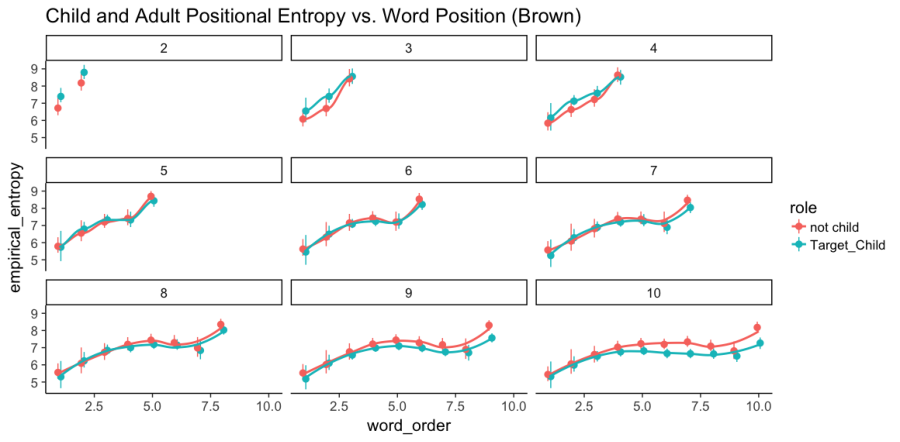
\includegraphics{figs/brown_PE-1} 

}

\caption[Brown corpus entropy]{Brown corpus entropy}\label{fig:brown_PE}
\end{figure*}
\end{CodeChunk}

\begin{CodeChunk}
\begin{figure*}[h]

{\centering 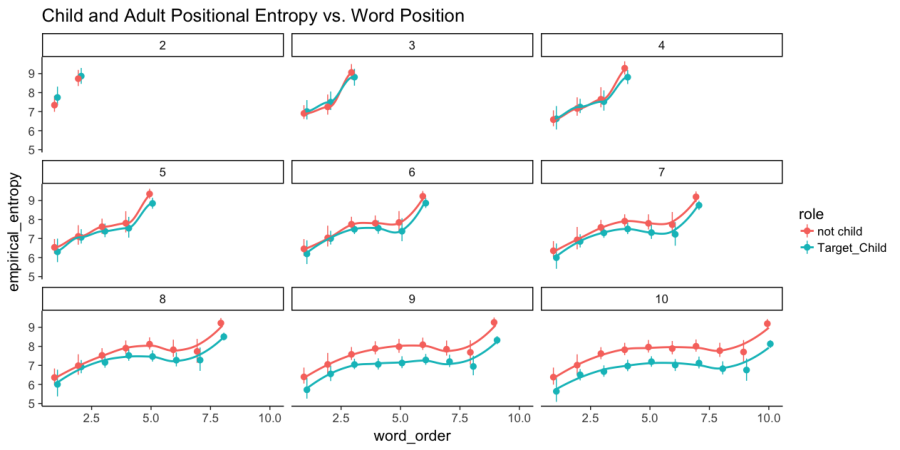
\includegraphics{figs/providence_PE-1} 

}

\caption[Providence corpus unigram entropy]{Providence corpus unigram entropy}\label{fig:providence_PE}
\end{figure*}
\end{CodeChunk}

We also ran this analysis on Spanish and Mandarin corpora from CHILDES.
We used the Shiro corpus for Spanish (Shiro, 2000), which contains
prompted narratives individually collected from over a hundred
Venezualan schoolchildren, half from high SES backgrounds and half from
low SES backgrounds. We used the Zhou dinner corpus for Mandarin Chinese
(Li \& Zhou, 2015), which contains dinner conversations between 5 to
6-year-old children and their parents collected in Shanghai.

For each corpus, we accessed transcripts of the corpus provided through
the TalkBank system and computed over Roman alphabet transcriptions or
transliterations of the original transcriptions. For Mandarin, we used
pinyin transliterations of the utterances in the corpus with demarcated
word boundaries, and for Japanese we used romanji (Roman alphabet)
transliterations of words in the corpus. The Chinese characters used for
writing Mandarin do not normally demarcate word boundaries by spacing
words apart, and for normal Chinese writing including spaces between
word boundaries can have a negative effect on reading times (Bai et al,
2008).

\begin{CodeChunk}
\begin{figure*}[h]

{\centering 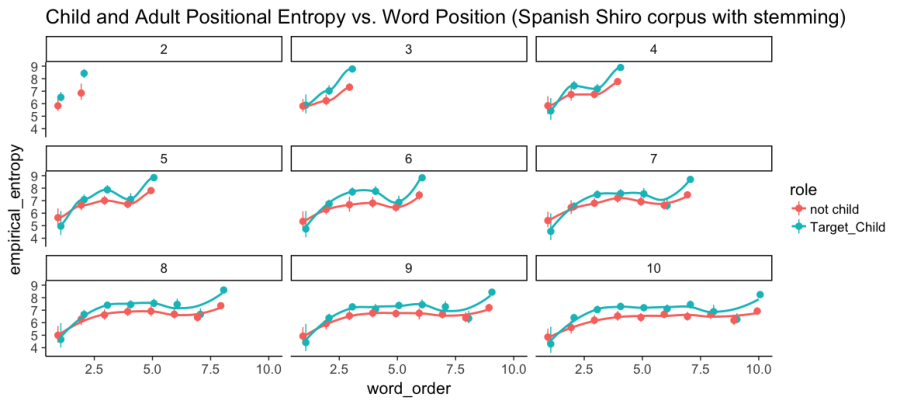
\includegraphics{figs/shiro_PE-1} 

}

\caption[Shiro corpus entropy]{Shiro corpus entropy}\label{fig:shiro_PE}
\end{figure*}
\end{CodeChunk}

\begin{CodeChunk}
\begin{figure*}[h]

{\centering 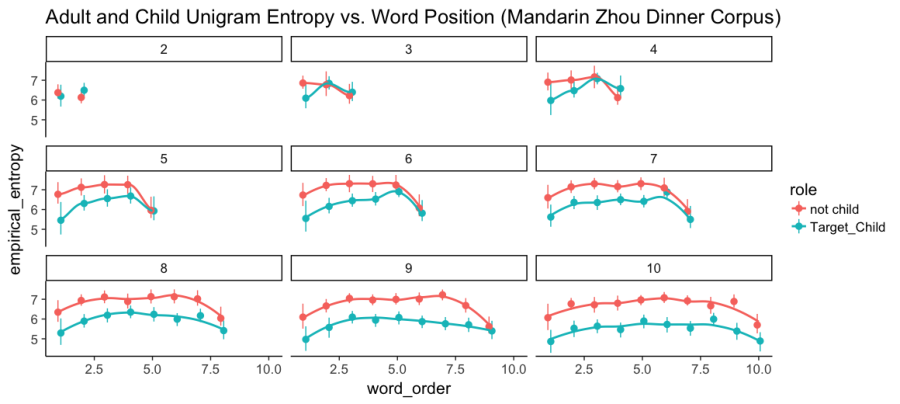
\includegraphics{figs/zhou_PE-1} 

}

\caption[Zhou Dinner corpus entropy]{Zhou Dinner corpus entropy}\label{fig:zhou_PE}
\end{figure*}
\end{CodeChunk}

\subsection{Results \& Analysis}\label{results-analysis}

The adult and child entropy curves track one another almost identically.
This is surprising because UID would predict that the young children in
the corpora who are not fully developed speakers would have more noise
in their distribution of information rates. This not only indicates a
robustness in the unigram entropy curve across speakers, but also across
ages and addressees. We also observed a robustness across corpora for
the same languages, and a robustness across utterance lengths within the
same corpus's entropy curve. This shows that the concept of an ``entropy
curve'' for a specific language is well-founded when considering speech
data.

We found a distinct three-step distribution for English and Spanish
CHILDES corpora, with a slight dip in the penultimate position of each
sentence. The final position of utterances in child-directed speech is
known to be important, dating back to Aslin (1993). The Mandarin corpus
entropy curve, by comparison, has a noticeably lower positional entropy
values in utterance-final positions than in utterance-penultimate
positions.

We attribute the penultimate dip in the English and Spanish entropy
curves to the fact that most of the utterances in the CHILDES English
and Spanish corpora we examined had a determiner such as ``the'' or
``a'' in the second-to-last position of utterances. The beginnings of
utterances in the English and Spanish CHILDES data were usually pronouns
or grammatical subjects, while the final words were grammatical objects
and had a great deal of variation in the exact word that appeared in the
utterance-final position.

These entropy curves are not what would be expected from UID. The
robustness of the three-step distribution for English and its
replication in Spanish do not resemble the affine function we would
expect from UID. The Mandarin entropy curve, which does not at all
resemble either the English/Spanish distribution or the predictions of
UID, suggests that the entropy curve can vary from language to language.
UID predicts that each language should have a similar distribution.

\section{Written data}\label{written-data}

The UID hypothesis also applies to written communication: we expect
people to communicate information at a uniform rate through writing as
well. We use Wikipedia as a source for written data, which provides two
advantages. One, the quantity of data in Wikipedia is large for each
language and two, there are hundreds of languages with Wikipedias. This
allows us to perform the entropy analysis on a much greater scale and to
directly compare the results of the entropy analysis on each language to
one another, and ultimately to predict what typological features of a
language help determine its entropy curve, if any. We will describe our
method of harvesting and distilling text data from each Wikipedia as
well as how we compare the entropy curves from each language to one
another.

\subsection{Methods}\label{methods-1}

Using Giuseppe Attardi's Wikiextractor tool
\footnote{https://github.com/attardi/wikiextractor}, we extracted the
text corpora for \(165\) languages from Wikipedia by downloading a
stored collection of Wikipedia entries in each langauge and randomly
selecting several thousand articles from each Wikipedia language. Each
language corpus was cleaned and limited to sentences between \(6\) and
\(50\) words. Similar to the data from CHILDES, we divided each corpus
by sentence length, and then computed the unigram entropy measure on
each word position within each sentence length.

To classify the unigram entropy curves of the different distributions,
we computed three slope treatments of each curve. In the \emph{absolute}
treatment, with sentence length denoted as \(n\), we computed the slope
between positions \(1\) and \(2\), positions \(2\) and \(3\), positions
\(3\) and \(n-2\), positions \(n-2\) and \(n-1\) and positions \(n-1\)
and \(n\). For the short utterances appearing the CHILDES speech corpora
we examined, these appeared to be important junctions in the
distributions, with a seeming plateau in the middle of the unigram
entropy curve for each of the language corpora we examined in CHILDES.

However, because the portion of sentences of length greater than \(10\)
in the Wikipedia corpora were significantly larger than the CHILDES
corpora, then we also computed relative slope treatments. In the
\emph{relative 5} treatment, we computed the slopes between \(0\%\) and
\(20\%\), \(20\%\) and \(40\%\), \(40\%\) and \(60\%\), \(60\%\) and
\(80\%\) and \(80\%\) and \(100\%\) of the relative word positions in
each sentence. When one of these percentages was not a whole number,
then the closest whole number position was used instead for slope
calculation. In the \emph{relative 10} treatment, we computed the slopes
between every \(10\%\) of the relative word positions in each sentence.
Each comparative slope within each treatment was averaged together
between different sentence lengths, for example in the \emph{relative 5}
treatment then all of the \(0\%\) to \(20\%\) slopes were averaged
together. This created three treatments for the entropy curve for each
langauge in the Wikipedia database.

For the German and Japanese entropy curves, we observed the same shape
for the text Wikipedia corpora entropy curves and the speech CHILDES
corpora entropy curves, supporting the argument for robustness across
text and speech.

\subsection{Results and Analysis}\label{results-and-analysis}

In the \emph{absolute} and \emph{relative 5} treatments, each language
is cast as a point in \(5\)-dimensional space. In the \emph{relative 10}
treatment, each language is cast as a point in \(10\)-dimensional space.
This allows for direct comparison using cosine similarity and moreover
for unsupervised clustering analysis to compare the results of the
Wikipedia entropy analysis to known typological features within the
langauges in the Wikipedia dataset. Using the R hclust package, we
performed a hierarchical clustering of the Wikipedia slope data within
each treatment. A subset of the results at a glance for the
\emph{absolute} treatment are below.

To determine which phonological, morphological and syntactic features
affected the embedding of a language in the Wikipedia dataset, we looked
at the list of \(144\) linguistic features in World Atlas of Language
Structures (Dryer \& Haspelmath, 2013). We limited the languages in the
WALS database to only those in our Wikipedia dataset and performed
missing-value imputation to obtain the features not coded in WALS for
the languages from Wikipedia.

One approach is to cluster the languages used in the Wikipedia analysis
on the basis of WALS features and then directly compare the WALS
clustering results with the results of the hierarchical clustering on
the Wikipedia slope data for each of the different treatments using
clustering similarity evaluation methods such as the Rand index (Rand,
1971). However, the problem then arises of which combination of WALS
features and how many features to include in the clustering analysis.
This is a computationally intractable operation. Additionallly, deciding
how many clusters to use in an unsupervised clustering analysis is an
unsolved problem in machine learning.

We instead check the effects of individual features on the embeddings of
languages in the different treatments. We computed pairwise cosine
similarity between each pair of language vectors within a treatment. For
a subset of WALS features which had values entered for most of the
languages we obtained from Wikipedia, we used a generalized linear model
to see whether the cosine similarity between languages mattered in
predicting if the languages shared the same value for a WALS feature. We
found this to be true.

\begin{CodeChunk}
\begin{CodeOutput}
\begin{table}[H]
\centering
\begin{tabular}{rrllrrrr}
  \hline
 & X & feature & term & estimate & std.error & statistic & p.value \\ 
  \hline
1 &   1 & 83A & cosine & 1.84 & 0.01 & 178.22 & 0.00 \\ 
  2 &   2 & 95A & cosine & 1.90 & 0.01 & 170.98 & 0.00 \\ 
  3 &   3 & 81A & cosine & 1.51 & 0.01 & 153.70 & 0.00 \\ 
  4 &   4 & 97A & cosine & 1.58 & 0.01 & 136.81 & 0.00 \\ 
  5 &   5 & 144A & cosine & 0.88 & 0.01 & 74.43 & 0.00 \\ 
  6 &   6 & 138A & cosine & 0.40 & 0.01 & 46.12 & 0.00 \\ 
  7 &   7 & 87A & cosine & 0.33 & 0.01 & 39.91 & 0.00 \\ 
  8 &   8 & 143A & cosine & 0.37 & 0.01 & 39.74 & 0.00 \\ 
  9 &   9 & 82A & cosine & 0.03 & 0.01 & 3.23 & 0.00 \\ 
   \hline
\end{tabular}
\end{table}
\end{CodeOutput}
\end{CodeChunk}

\section{Conclusions}\label{conclusions}

In this paper we have explored the differences in rate of information
transmission among spoken child-adult conversational corpora in several
languages and text corpora pulled from Wikipedia for well over a hundred
other corpora. We have seen that the entropy curve, a representation of
information at each position of an utterance without regard to context,
varies from language to language and is predicted by a subset of
syntactic, phonological and morphological features in a language. We
have provided evidence against the Uniform Information Density
hypothesis and provided an alternate explanation for the rate at which
information is encoded and transmitted in human communication, namely
one that is robust across corpora, language dependent and arises from
the features of the language.

A large volume of research has indicated the effects of surprisal on
fixation duration during eye-tracking studies: higher surprisal of a
word corresponds to higher fixation duration. The \emph{wrap-up effect}
is a popular hypothesis within the eye-tracking community. The
hypothesis states that, in written text, sentence-final words are
processed more slowly on average then sentence-medial or
sentence-initial words, due to readers integrating information from the
entire sentence in order to form a final, coherent thought expressed by
the sentence, among other reasons. The wrap-up effect is drawn from
evidence in English, German and Dutch, all of which are languages with a
large final increase in their entropy curve from our study. We aim to
see in the future if as a consquence of our work in this paper, the
wrap-up effect falls out from the final jump in the entropy curves in
some languages.

\setlength{\parindent}{-0.1in} \setlength{\leftskip}{0.125in} \noindent

\bibliographystyle{apacite}


\end{document}
